
\chapter{The Bharatanāṭyaṃ \textit{Yajña}}\label{intro}

\Authorline{Prakruti Prativadi}


\section*{Abstract}

Bharatanāṭyaṃ (referred to in the past as Sadir, Dāsiāṭṭaṃ and Karnāṭakaṃ) was historically practiced, protected and nurtured in present day Tamil Nāḍu and Karnāṭaka. Bharatanāṭyaṃ is an embodied manifestation of Vedic philosophy and South Indian culture. Despite the ban on Devadāsi-s and the performance of Bharatanāṭyaṃ in temples due to colonial rulers, Bharatanāṭyaṃ has now achieved a pan-Indian and global popularity.

From the perspective of a practicing Hindu teacher and dancer, this paper discusses how Bharatanāṭyaṃ, regardless of where it is performed, is not merely art but a sacred Hindu \textit{sādhanā}, requiring \textit{bhakti, śraddhā} and most significantly, \textit{sattva} on the part of the dancer. We discuss how the performance is a Hindu ritual of \textit{yajña} per the Nāṭyaśāstra. The purpose of this ancient art form is not only to produce an aesthetic effect but to transform the consciousness of the onlooker to experience the \textit{Paramātman} through \textit{Rasa}. Classical dance derives from the four Veda-s and is thus \textit{Nāṭyaveda}; the Vedic philosophy and world view, and Hindu rituals are inseparable from the dance.

The aesthetic theory of the Nāṭyaśāstra by Bharatamuni is the foundation of Bharatanāṭyaṃ. We discuss the specific requirements that must be satisfied for a subject to qualify as a Bharatanāṭyaṃ dance. Furthermore, we examine two recent drifts in the Bharatanāṭyaṃ domain. The first is the removal of the intrinsic sacred Hindu rituals, symbols, themes, and philosophy from dances to re-fashion Bharata\-nāṭyaṃ as non-sacred. The second is the use of Christian imagery and ideology in Bharatanāṭyaṃ dances either alongside Hindu themes or by completely replacing Hindu themes. We analyze how these drifts do not meet the necessary requirements to qualify as Bharatanāṭyaṃ dance and are antithetical to its nature.


\section*{Introduction}

In recent years, Bharatanāṭyaṃ has seen an extraordinary increase in popularity in India and the globe; it is danced by a diverse group of people from wide-ranging educational, linguistic, racial, religious, and economic backgrounds. However, the understanding of the dance, and therefore its authentic practice, in many cases is diluted and abridged. Bharatanāṭyaṃ, once again stands at a turning point in its future; over a century ago, it was outright banned due to colonial bigotry, but now its very popularity has brought about erosion and drift from its authentic form. Bharatanāṭyaṃ has endured for millennia; however, to safeguard its future, guru-s and the classical dance community need to ensure that the fundamental purpose and nature of the art is correctly understood and practiced, without dilution and exploitation for material purposes.

Currently, Bharatanāṭyaṃ is most commonly seen through one of these lenses:

\begin{enumerate}[{\rm 1)}]
\itemsep=0pt
\item A pleasant entertaining dance form presenting some cultural customs and stories/epics of India.

 \item A non-sacred art medium in which one can voice any narrow viewpoint or opinion.

 \item A dance that can be used to inculturate Christian theology and doctrine for the purposes of evangelization. 

 \item The original lens of the Nāṭyaśāstra and other treatises wherein Bharatanāṭyaṃ is a \textit{Yajña} and an offering to the Hindu Gods so the dancer and audience can come closer to Brahman and \textit{Sat-Cit-Ānanda}.

\end{enumerate}

Presently, many Bharatanāṭyaṃ dancers think that it is only an artistic medium. However, the ancient treatises, guru-s and exponents have defined Bharatanāṭyaṃ as the following:

\begin{enumerate}[{\rm 1)}]
\itemsep=0pt
\item A physical manifestation and embodiment of Vedic knowledge and philosophy (as explicitly stated in the foundational dance, music and drama treatise, the \textit{Nāṭyaśāstra}, and further reiterated in the \textit{Abhinavabhāratī} and \textit{Sangīta Ratnākara}).

 \item An embodiment of Hindu metaphysics and is indivisible from it. Bharatanāṭyaṃ dances must have certain Hindu metaphysical prerequisites which are inextricable from its technical dance movements and dance numbers, that must be satisfied by the dancer.

 \item A \textit{sādhanā} that requires the dancer to immerse themselves for many years with the utmost \textit{Śraddhā} and \textit{Bhakti}, and the performance Hindu rituals and \textit{pūjā} to Hindu Gods is an inseparable part of this \textit{sādhanā}.

 \item As stated in the Nāṭyaśāstra, Bharatanāṭyaṃ must awaken the \textit{Rasa} experience, \textit{Rasa} experience is similar to the experience of \textit{Brahman} (Pande 2009: xxii).

\end{enumerate}


\section*{Hindu Worldview}

Bharata wrote the Nāṭyaśāstra from his insider worldview, i.e. the Hindu Vedic worldview, therefore, it is only the Vedic worldview in which Bharatanāṭyaṃ can be understood and practiced. A person who has practiced Bharatanāṭyaṃ as a \textit{sādhanā }naturally understands it within this framework. His or her \textit{anubhava }from this\textit{ sādhanā }is invaluable in understanding the practical and theoretical facets of Bharatanāṭyaṃ. On the other hand, a person who dances Bharatanāṭyaṃ as merely a non-sacred art for entertainment lacks this intrinsic understanding. Here by \textit{anubhava} we do not mean ‘experience’ as it is often mistranslated, but we mean the direct knowledge of the \textit{ātmān, ātmānubhava }is direct self-knowledge (Swami Dayananda Saraswati 2007). This \textit{ātmānubhava} comes from being immersed in Bharatanāṭyaṃ, its customs, philosophy, and rituals with full \textit{Śraddha} and \textit{Bhakti}, ultimately leading the \textit{jīvātma} to become one with the \textit{Paramātma}, as with any Hindu \textit{sādhanā}. In effect, Bharatanāṭyaṃ is a form of embodied knowing (Malhotra 2011: 5-6).

The birth of Indian dance and Bharatanāṭyaṃ is within the Hindu world view. This is the lens in which the aesthetics and philosophy of Bharatanāṭyaṃ reside. The dances of Bharatanāṭyaṃ and its rituals make sense only when this view is espoused.

The Hindu world view contains the following metaphysics:

\begin{enumerate}[{\rm 1)}]
\itemsep=0pt
\item All living beings i.e. \textit{jīvātman-s} have the \textit{Paramātman} within them. 

 \item The \textit{ātma} was never created and can never be destroyed and is changeless.

 \item The \textit{Paramātman} lives in every living being and pervades every space. They are inseparable. 

 \item The earth, nature, water, space, planets and animals are all sacred Hindu Gods, Goddesses, and \textit{Devatā-s}. The earth is the Goddess Bhūmidevī, fire is the \textit{Deva }Agni, water is Varuṇa, rain is Indra, wind is Vāyu, death, or the “ordained time” is revered as Yama. The directions are also \textit{Devata-s}; all the elements are sacred. Thus, in the Hindu worldview there is nothing in conflict, nothing is intrinsically evil, and nothing needs to be conquered. 

 \item Humans (\textit{jīvātman-s}) are limited (due to previous \textit{karma-s}) and can overcome this limited state through \textit{Brahman} realization through their own efforts without being shackled by dogma and doctrines.

 \item \textit{Brahman} is the true Self which is the goal of life and \textit{mokṣa} gives Brahman knowledge. It is important to note that Brahman, \textit{Paramātma}, or Īśvara, or Kṛṣṇa or any of the Hindu deities are not the same as the God defined in the Abrahamic traditions.

 \item \textit{Rasa}, \textit{Bhāva }and \textit{Sattva} are a means to unite with the \textit{Paramātma}.

\end{enumerate}

The above metaphysics guides the dances and customs of Bharata\-nāṭyaṃ. We sanctify the stage, perform a ritual \textit{Namaste} to the earth (to Goddess Bhūmidevī) and in the dance itself we acknowledge all the directions. These deities are unique and cannot be replaced arbitrarily by others.

Many Sanskrit words have no accurate translation in English. This is crucial to understanding Bharatanāṭyaṃ in its own terms and in its own domain without erroneously mapping English words that do not convey the same meaning as the original. As we shall see in this paper, words such as \textit{rasa}, \textit{yajña, bhāva, abhinaya, sattva, bhakti, sraddhā, mudra,} and \textit{sahṛdaya} among others, do not have one-to-one translations in English. The propagation of these erroneous translations inhibit the understanding of these concepts in Bharatanāṭyaṃ.

Bharatanāṭyaṃ rituals and customs can now be understood within this world view. Some of the important mandatory rituals in a performance are:

\begin{enumerate}[{\rm 1)}]
\itemsep=0pt
\item A “\textit{Namaste”} is performed to the \textit{Paramātman }and also to \textit{Bhūmidevī} since the dancer is dancing on this Goddess \textit{Bhūmidevī} and seeks her forgiveness for touching her with the feet. This Bharatanāṭyaṃ \textit{Namaste }must be done prior to and at the conclusion of a performance, a class and also daily practices.

 \item Prior to \textit{nāṭyāraṃbhaṃ }(start of learning Bharatanāṭyaṃ), a \textit{pūjā }to Sarasvati, Gaṇapati, Naṭarāja must be done. This Hindu \textit{pūjā }is not for just seeking blessings but to offer (\textit{samārpaņam}) the dances and their \textit{phala }to these Hindu Gods.

 \item The stage must be made into a Hindu sacred space, by offering Hindu \textit{pūjā }to Gods such as Sarasvati, Lakṣmi, Naṭarāja, Viṣṇu and Gaṇapati. A \textit{pratiṣṭhāpana }of these \textit{mūrti}-s is performed on the stage and a \textit{pūjā }and \textit{ārati} performed with appropriate Hindu \textit{mantra-s}.

 \item Namaste to the \textit{guru} and \textit{guru} \textit{paramparā.}

 \item During Navaratri’s Sarasvati \textit{pūja} day, the dance bells and \textit{naṭṭavāńgaṃ} are placed before Sarasvati and \textit{pūjā }done to them.

 \item \textit{Pūjā} to the dance bells and \textit{naṭṭavāngaṃ} and \textit{arcanā} in a Hindu temple is performed prior to any Bharatanāṭyaṃ performance.

\end{enumerate}

As we shall see, in the next sections, there is a precedent for all these rituals in the Nāṭyaśāstra and they unify the entire Bharatanāṭyaṃ performance experience for both the dancer and the audience.


\section*{Origin of Indian Dance}

As with any serious subject, the sincere and honest approach to accurately comprehend and practice Bharatanāṭyaṃ is to go back to its foundation which is the Nāṭyaśāstra and other later treatises like \textit{Abhinavabhāratī}, and \textit{Sańgīta Ratnākara}. The importance of the Nāṭyaśāstra cannot be overstated. The Nāṭyaśāstra, written more than 2500 years ago, by Bharata, is the oldest extant treatise on dramaturgy, dance and music and still is the authority today. The Nāṭyaśāstra explains the aesthetic philosophy and metaphysics of Indian dance. Bharata connects the art of movement of the body to the mind, intellect and most significantly, to the human consciousness. Bharata referenced earlier Hindu works on dance and drama to compile the Nāṭyaśāstra. The Nāṭyaśāstra contains not just the technical movements and other technical practical details but most importantly, explains the origin of the Nāṭyaveda and the reason Indian dance is practiced and performed. This informs and guides the practice of all Indian ancient dances including Bharatanāṭyaṃ for more than two millennia. 

To a practitioner of Bharatanāṭyaṃ who has read and understood the Nāṭyaśāstra and Abhinavabhāratī and Sańgīta Ratnākara, it is obvious that Bharatanāṭyaṃ derives from these. The \textit{hastamudra-s}, stances, basic steps and movements of each body part such as the head, face, hands, arms, feet, legs, torso etc. described in the Nāṭyaśāstra are still practiced today and though the \textit{aḍavu-s }and \textit{jati-s }evolved from the \textit{karana-s} and \textit{angahāra-s}, they are analogous. The technique and theory of \textit{abhinaya} and their use in evoking \textit{bhāva-s} and \textit{rasa }are remarkably continuous since the days of the Nāṭyaśāstra.

Indian dance, drama and music derived from the Veda-s and represent the thought system and knowledge of the Veda-s. In an extremely significant dialogue in the Nāṭyaśāstra, Brahmā is asked by the Ṛṣi-s to create an art that will contain all the knowledge of the Veda-s and be accessible to all people, of every \textit{varṇa}. In order to do so, Brahmā performs \textit{tapas} on the four Veda-s and then creates a fifth, the Nāṭyaveda which is for the benefit of all, conducive to \textit{dharma}, containing the wisdom and guidance of the \textit{śāstra-s }and comprised of \textit{itihasa-s} (Nāṭyaśāstra I.15,16). Brahma took the \textit{pāṭhya} (recitative) from the Ṛg Veda, \textit{gīta} (music) from the Sāma Veda, \textit{Abhinaya} from the Yajur Veda and \textit{Rasa} from the Atharva Veda to create the Nāṭyaveda directly connected to the Veda-s and the Upaveda-s (\textit{Nāṭyaśāstra} I: 17,18).

Brahma is also concerned that this new Veda should be practiced and passed on to those who will practice it authentically without deviation. After asking Indra to find suitable persons who are hardworking, knowledgeable, can fulfill \textit{vrata} and are capable of protecting and practicing the Nāṭyaveda, he decides to entrust the Nāṭyaveda to Bharata and his sons.(\textit{Nāṭyaśāstra} I. 23-25)

Bharata explicitly states that Nāṭyaveda was created to nurture and uphold Dharma: (Nāṭya) teaches \textit{dharma} to those who are against it, gives relief to those who are afflicted or fatigued, brings determination to the sorrowful, enlightens those with poor intellect, brings courage to the cowardly, gives enthusiasm to the heroic, teaches love to those who are eager for it, rebukes the ill-mannered, promotes will-power in the disciplined, gives diversion to the noble and brings happiness, good counsel and knowledge to all. (\textit{Nāṭyaśāstra} 1:108-115)

After the first dance, the illustrious among the assembly gave gifts to the dancers, singers and actors. This is an ancient custom of India that was in practice for many years until recently. The rich people compensated the artists and the poorer classes could enjoy the performance free of charge. Nowadays this has been replaced by charging audiences prior to a performance. (Kumar 2006: 26)

The construction of the theater is very detailed and precise measurements for different types and sizes are given. \textit{Devatā-s} are then placed in each part of the theater, for example, \textit{Agni} on the stage, \textit{Candra }in the main building, \textit{Marut-s} the corners, \textit{lokapāla-s} its sides, and \textit{Yama} the door. \textit{Brahmā} is seated in the middle of the stage, which is why flowers are offered there. (Nāṭyaśāstra 1:82-94) This shows that the theater itself is like a Hindu sacred space, much like a \textit{Yāgaśāla}.

Nowhere in the Nāṭyaśāstra does it say that \textit{Nāṭya} is just art in which any and all opinions and petty viewpoints can be propagated. By Bharata’s explanation we see that Nāṭyaveda is a manifestation of the knowledge in the Veda-s and is a complete experience that involves more than just providing entertainment or a worldly diversion to the audience. Indian dance was created to give knowledge of Vedic principles and benefit everyone in society. Significantly, we see that Indian dance is not just for the elite or the rich, is for the enjoyment and advantage of everyone from all parts of society. The dance is a transformative experience, like all Hindu customs and rituals. The four \textit{Puruśārtha-s} of \textit{dharma, artha, kāma }and \textit{mokṣa} are enacted during the dances. The \textit{Puruśārtha-s} are of significance because dharma is the guiding and unifying factor for the attainment of \textit{artha, kāma }and \textit{mokṣa}. By viewing the \textit{Puruśārtha-s}, the onlooker experiences \textit{Bhava-s} and ultimately \textit{Rasa}. Per the Nāṭyaśāstra and \textit{Abhinavabhāratī}, \textit{Rasa} is the paramount aim of Indian dance, drama and music, because it is through this \textit{Rasa} experience that the onlooker can experience something akin to Brahman.


\section*{\textit{Rasa}}

To understand the Hindu metaphysics embedded in the aesthetics of Bharatanāṭyaṃ we will need to examine \textit{Rasa} and \textit{Abhinaya}. A unique feature of Bharatanāṭyaṃ and Indian Aesthetics is \textit{Rasa}. \textit{Rasa} does not have a direct translation in English, in this context. In aesthetics, \textit{Rasa} does not translate to feeling, or emotion or mood, or essence, or sentiment. \textit{Rasa} is a supreme aesthetic experience that is similar to \textit{Brahmānanda}. As Abhinavagupta states, \textit{Rasānanda} is similar to \textit{Brahmānanda} - the bliss of Brahman knowledge. \textit{Rasa} is a consciousness-elevating state that can be experienced by a \textit{sahṛdaya}. Remarkably, \textit{Rasa} cannot be understood solely in the intellectual and emotional domains. \textit{Rasa} involves the mind, intellect and the \textit{jīvātman} (consciousness), and must be experienced. \textit{Rasa} is paramount. \textit{Rasa} is not guaranteed in any given artistic work and all stories or themes cannot generate the powerful \textit{Bhāva-s}, \textit{Vibhāva-s, Anubhāva-s}, and \textit{Sthāyi bhāva-s} necessary to generate \textit{Rasa}. It is something that must be carefully generated and is born only if meticulously chosen conditions arise in a dance performance.

\textit{Rasa} does not exist in isolation, \textit{Rasa}-s are the culmination of a complex process that involves the generation of varieties of \textit{bhāva-s}, which are mental and emotional states that vary depending on the character and circumstance. There are forty-nine \textit{bhāva-s }consisting of thirty-three \textit{Vyabhicāri} (impermanent) \textit{bhāva-s}, eight \textit{Sāttvika bhāva-s} (with \textit{Sattva}) and eight \textit{Sthāyi} (permanent) \textit{bhāva-s}. \textit{Rasa} is born as result of all these \textit{bhāva-s}- the \textit{Vibhāva-s}(determinants), \textit{Anubhāva-s} (consequent reactions), \textit{Vyabhicāri, Sāttvika} and \textit{Sthāyi bhāva-s }emerging first. The organic and natural coming together of these results in the \textit{Rasa experience }of the spectator. It is not an afterthought or an automatic outcome. The following diagram summarizes the awakening of \textit{Rasa} (Prativadi 2017:46).

\begin{figure}[!htbp]
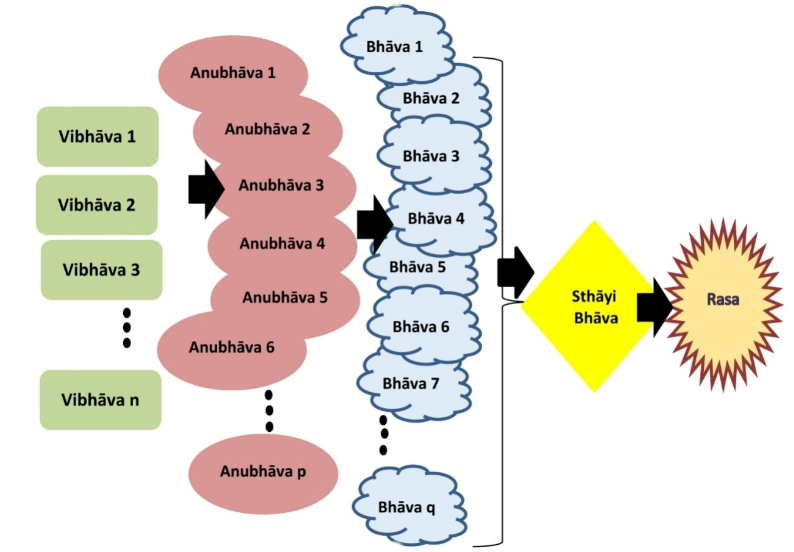
\includegraphics[scale=1.21]{"images/11-01.jpg"}
\end{figure}

The dancer must generate these \textit{Bhāva-s} and \textit{Vibhāva-s} in a genuine manner so that \textit{Rasa} is born. The subject and themes she chooses to do this are of supreme importance. The limited-self disappears to reveal the more pervading \textit{Paramātma}. \textit{Rasa} is permanent; it touches and elevates the \textit{jīvātman}. That is why Bharata emphasizes that a \textit{sahṛdaya} is best suited to experience \textit{Rasa}. \textit{Rasa} is of such significance, that Bharata himself declared: “There can be no meaningful communication without \textit{Rasa}.” The challenge to the artist is to be able to produce this \textit{Rasa} experience for all members in their audience in their performances.

Per the Nāṭyaśāstra, a dance, drama, or music performance that does not generate \textit{Rasa}-s and is not offered to the Hindu Gods is not really art and is \textit{nīca }(vulgar). This kind of performance will not benefit either the audience or the performers. \textit{Rasa} is not limited to the stage or court; \textit{Rasa} comes from a set of conditions the dancer creates. \textit{Rasa} is born after the generation of many and varied \textit{bhāva-s} (mental and emotional states) that differ, based on the character and circumstance.

The \textit{Rasa} experience stays with the audience for some time even after the performance has concluded; the audience wants to experience it again. During the \textit{Rasa} experience, the very consciousness is transformed to reflect the true inner Self. The concept of \textit{Rasa} is ancient and found in the Veda-s and Upanishad-s. The Taittirīya Upaniṣad declares that: \textit{Raso vai Saḥ}: \textit{Rasa} (is) Him (Brahman).

\newpage

\textit{Rasa} is not isolated to dance, but also exists in poetry, music and drama. The dances of temples, performed by devadāsi-s and, in some cases, even temple priests, also have the same goal of generating \textit{Rasa} in the onlooker because these dances are not just rituals, they generate \textit{Bhāva-s} which result in \textit{Rasa}; the devadāsi-s also offered their dances to the Hindu Gods, which is the same motive of the dance performed on the \textit{raṅga} (stage) described in the Nāṭyaśāstra. There is no difference in purpose between the dance described in the Nāṭyaśāstra and the dance of the temples.

Thus, \textit{Rasa} is neither trivial nor commonplace. Every single element of the dance, including the music \textit{rāga-s, tāla-s, aḍavu-s }and even the dancer’s costume, makeup and accessories all come together to generate the \textit{Rasa} experience. Originally, \textit{karaṇa-s }and \textit{aṅgahāra-s }(analogous to \textit{aḍavu-s} and \textit{jati-s} of Bharatanāṭyaṃ) produced \textit{Rasa}. Thus, \textit{Rasa-s} should be generated by every aspect of the dance, not just \textit{Abhinaya }but also by \textit{nṛtta} and \textit{nṛtya}.


\section*{\textit{Abhinaya}}

\textit{Abhinaya} is not just the ordinary enactment of stories and characters but the exalted, idealized and glorified re-enactment of stories and characters. \textit{Abhinaya} has been often mistranslated into mime and pantomime and is neither of these. \textit{Abhinaya} literally means to carry the performance to the audience. This re-enactment generates \textit{bhāva-s} and \textit{Rasa-s} which are readily received and experienced by the \textit{sahṛdaya}. By watching the re-enactment of these stories and characters, which are carefully chosen and which enact the four \textit{Puruṣārtha-s} of \textit{dharma, artha, kāma} and \textit{mokṣa}, the audience is removed from their mundane day-to-day troubles and problems. The audience forgets the petty limited everyday world and experiences something greater, a limitless Self (\textit{Paramātman}) where the ego disappears and a permanent innate joy is experienced. The dancer must, in effect, disappear from the performance, her ego must not be apparent. For instance, a dancer cannot effectively embody Ānḍāl or dance the \textit{Vāriṇaṃ Āyiraṃ }without shedding her own persona. The dancer’s petty egos, problems and grievances should not be visible in such a performance since, if they were, the performance would not be able to produce the desired \textit{Rasa} experience in the onlooker. Indian dance has survived for millennia because of this unique characteristic. Indian aesthetic theory is unique in that the \textit{rasa} concept does not have parallels in aesthetic theories of other world cultures. \textit{Abhinaya} requires \textit{Sattva} and \textit{Sāttvika} state of mind to successfully generate \textit{bhāva-s} and \textit{rasa-s}.

\textit{Abhinaya} consists of four types:

\textbf{\textit{Āṅgika Abhinaya}:} Using the body, including the arms, hands, feet, legs, torso, face, and head in dramatic representation.

\textbf{\textit{Vācika Abhinaya}:} Dramatic portrayal through the use of speech, in Bharatanāṭyaṃ Vācika \textit{Abhinaya} consists of the songs and compositions that are danced.

\textbf{\textit{Āhārya Abhinaya}:} Consists of make-up, jewelry, flowers, props and accessories used by the dancer to aid in dramatic portrayal.

\textbf{\textit{Sāttvika Abhinaya}:} Emoting and portrayal of characters and situations through \textit{Sattva}., (Sattva is a non-translatable)

All these types of \textit{Abhinaya} are essential to generate the Bhāvas and awaken \textit{Rasa} in the audience. Amongst these, however, the more intangible and indefinable type is undoubtedly \textit{Sāttvika Abhinaya}. \textit{Sāttvika Abhinaya} is portrayal that is full of \textit{Sattva}. This is a crucial ingredient, because it is required to genuinely embody the Bhāvas that will generate Rasas.

Bharata states that a successful performance is not one in which the dancers win awards or gain materially but one in which the \textit{Rasa} experience was powerful and experienced by the audience. This is the measure of \textit{siddhi} (success) that Bharata emphasizes.


\section*{\textit{Sattva}}

\textit{“One must take particular care of Sattva… for Abhinaya resides in Sattva” -Nāṭyaśāstra Sāttvika Abhinaya}, as the Nāṭyaśāstra states is an intangible but vital element in generating the \textit{Bhāva-s} and \textit{Rasa-s}. Generating \textit{Rasa} in the audience is not a simple task. The dancer must possess the technical skill, imagination, intellect and a certain state of mind to be able to embody the characters, stories, and movements that evoke \textit{bhāva-s} and \textit{rasa}. According to the Nāṭyaśāstra and the \textit{Saṅgīta Ratnākara}, in order to evoke \textit{Rasa} in the audience, the dancer’s mind and consciousness must be in a state of \textit{Sattva}.

\newpage

\textit{“Sattva can only be accomplished by a tranquil, peaceful and concentrated mind” -Nāṭyaśāstra} Bharata and Abhinavagupta emphasize that a performance without \textit{Sattva} will not move the audience and will not produce \textit{bhāva-s} and \textit{rasa-s}, and thus, will be unsuccessful and meaningless. 

\textit{Sattva} is a Sanskrit word that has no direct translation in English or non-Indian languages. Interestingly, even Indologists such as A.B. Keith agreed that “\textit{Sattva”} has no translation. \textit{Sattva Guṇa} is one that is bright, pure, luminous, buoyant, happy and stainless. Under the influence of \textit{Sattva}, the mind is calm, never agitated, filled with \textit{Śraddhā}, steady, and reflects the Self (Brahman). A person with a \textit{Sāttvic} mind renounces the results of his or her actions; in other words, actions motivated by \textit{Sattva} are offered to the Supreme. As the Nāṭyaśāstra makes clear in the very first chapters, Nāṭya, which consists of Indian classical dance, drama and music, whether performed on a stage or in a temple must be an offering to the Hindu Gods, Goddesses and \textit{Devata-s}. \textit{Rajas} is agitation, activity, pain, egotistic, seeking sense-pleasures, and \textit{Tamas}, is dark, inert, lazy, indifferent and exhibits low passions and tendencies. Our actions are controlled and directed by the mind which exhibits a combination of these three \textit{guṇa-s}.

When the mind is purified, \textit{Rajas }and \textit{Tamas} are not present and the mind is \textit{Sāttvic} and in a state of \textit{Śānti} and\textit{ Ānanda }and is able to reflect the Self (Brahman). The \textit{Rasa} experience itself, is likened to the bliss of Brahman knowledge. \textit{Sattva} modifies the consciousness to bring out \textit{Rasa}. In the Nāṭyaśāstra, Bharata describes eight \textit{Sāttvika} \textit{bhāva-s} which are: paralysis, sweating, goose-bumps, change in voice, trembling, pallor, weeping and fainting. According to Bharata, these \textit{Sāttvika bhāva-s} give genuineness and realism to the dance and make the audience to become one with the performance, hence generating \textit{bhāva-s} and \textit{Rasa}. Bharata states that in order to embody the \textit{Sāttvika bhāva-s}, the dancer’s mind must be in a state of \textit{Sattva} – purified of the \textit{Rājasic} and \textit{Tāmasic} attributes. It is important to note that the dancer’s mind must be in a state of \textit{Sattva} even when the dancer is portraying characters or \textit{bhāva-s} that are not \textit{Sāttvic}. The dancers themselves are not experiencing the \textit{bhāva-s}, however, in order for their portrayal to be realistic and to convey the \textit{bhāva-s} and generate Rasa in the spectator, the dancer’s mind would have to be in a state of \textit{Sattva.}

Thus, a prerequisite to an outstanding dance performance is that the dancer must accomplish a state of \textit{Sattva} before the performance and maintain this state of mind during the performance to generate \textit{Rasa}. How does the dancer go about preparing the mind to be \textit{Sāttvic}? It is not just a matter of motivating oneself through pep talks or having a few minutes of quiet solitude before the performance. These, of course, can help and all Bharatanāṭyaṃ dancers, to some extent, will use these techniques. But to have the mind in a state of \textit{Sattva} prior to and during the performance, the dancer would need more than just motivational techniques, and Bharata addresses this in the Nāṭyaśāstra.


\section*{\textit{Yajña}}

The third chapter of the Nāṭyaśāstra is dedicated to explaining, in detail, a series of \textit{pūjā-s} and a \textit{homa} that the dancer and musicians should perform. In these instructions, Bharata clearly states that these \textit{pūjā-s} and \textit{homa} are the equivalent of performing a \textit{Yajña} and will help the dancer achieve a calm mental and conscious state necessary for a successful performance. \textit{Siddhi} or success in a performance, per Abhinavagupta and Bharata, does not mean winning banners (prizes) or material objects, but \textit{Siddhi} of the performance occurs if the audience witness compelling \textit{Bhāvas} and experience the different Rasas. 

Therefore, these \textit{pūjā-s} and \textit{homa} are not robotic superstitious ritualistic acts; they are a science of connecting the \textit{jīvātman} to the \textit{Paramātman}. They are an offering and a means for the artistes to transform and purify their inner-selves to be \textit{Sāttvic. }In these pre-performance Hindu sacred activities, Bharata details how the \textit{raṅga} (stage) must be constructed according precise measurements depending on the type of \textit{Nāṭya }to be performed. Significantly, the \textit{Vedī} (altar) of a \textit{Yajña} must also be constructed in a precise shape with exact measurements depending on the type of \textit{Yajña} performed. Bharata then specifies how the dancer must sanctify this stage, and even the entire theatre where that audience will be seated, the dancer should then do a \textit{Pratiśṭhāpana} (sacred installation) of the Hindu Gods on the stage, and do a \textit{pūjā }to each one of these deities in a certain order and with particular sacred \textit{mantra-s}. The dancer must sprinkle sanctified water on each limb to purify the body and must partake of the \textit{pūjā }and \textit{homa} with the utmost \textit{śraddhā} and \textit{bhakti }in order to bring his or her mind into a state of \textit{Sattva}. These actions along with their subtle effects will give \textit{siddhi} by preparing the dancer to be capable of a performance that is rich in \textit{bhāva-s} and \textit{rasa-s}. These performances are a few hours long and in some classical dances, like Kathakaḷi and Yakṣagāna, last through the night, so the dancer needs to muster tremendous energy, enthusiasm and concentration. The musicians too must perform a \textit{pūjā }to their instruments. In effect, the stage and entire theater (where the audience are seated) become a temple, with the consecration of deities and \textit{pūjā-s} and finally with the performance of the \textit{homa}. Bharata instructs that the point of doing the \textit{pūjā-s} and \textit{homa} are to offer the performance (dance) itself to the \textit{Devatā-s}. Not performing the \textit{puja-s} to Hindu deities with a \textit{Sāttvika} mind will result in not only failure of the performance, but and accrue bad \textit{karma}. This is perhaps vital in understanding that Indian \textit{Nāṭya} is indeed a \textit{Yajña}, and is meaningless otherwise.

A few samples from the Nāṭyaśāstra Chapter III that illustrate this view are as following –

\begin{verse}
\textit{padmopaviṣṭaṃ brahmāņaṃ tasya madhye niveśayet |}\\\textit{ādau niveśyo bhagavānsārdhaṃ bhūtagaņaiḥ śivaḥ || 24||}\\\textit{naaraayaņo mahendraśca skandaḥ sūryo’śvinau śaśī |}\\\textit{sarasvatī ca lakṣmīśca śraddhā medhā ca pūrvataḥ || 25 ||}
\end{verse}

(Once the stage and auditorium/theatre hall is constructed, all the gods are to be invoked and placed reverently with due procedure and location.) “In the middle is to be established Brahmā seated on the lotus after establishing Bhagavān Śiva along with his hordes of Bhūtas (24). Towards the eastern direction should be placed Nārāyaņa, Mahendra, Skanda, Sūrya, Aśvin-s, the Moon, Sarasvatī, Lakṣmī, Śraddhā and Medhā (25).”

\begin{verse}
\textit{na tathā pravahatyagniḥ prabhañjanamīritaḥ |}\\\textit{yathā hyaprogastu prayukto vahati kṣaņāt || 101||}\\\textit{śāstrajñeņa vinītena śucinā dīkṣitena ca | }\\\textit{nāṭyācāryeņa śāntena kartavyaṃ raņgapūjanam || 102||}
\end{verse}

“Fire fanned by the breeze does not burn as fiercely as a performance without proper procedure would immediately.(101) The stage worship should be performed by a nāṭyācārya (guru or stage director), who is endowed with learning, humility, pure in heart and behavior, pious, of peaceful temperament and initiated in the śāstras and vows (dīkṣā).( \textit{Nāṭyaśāstra} III. 102)” 

 Among these preliminary activities, the \textit{homa} (similar to a \textit{Yajña}) is of distinct interest and serves a special purpose. \textit{Yajña-s} are ancient Vedic practices that are transformative and have subtle effects on the consciousness of the performer. \textit{Homa} derives from and is an adaptation of a \textit{Yajña}, but a \textit{homa} is performed in \textit{pūjā-s }to specific Gods. Both feature a specifically constructed altar, sacred fire and sacred materials. \textit{Yajña} comes from the root word \textit{Yaj} which means offering, reverence, adoration and bestowing. A \textit{Yajña} and \textit{homa,} are \textit{tyāga }(offering) of \textit{dravya} (special sacred Sattvic material) to the \textit{Devatā-s}. They are complex activities that have subtle and powerful effects. Every offering during the \textit{Yajña} and \textit{homa} results in \textit{apūrva} \textit{Śakti}, which is a subtle effect and hidden power of an action (\textit{karma-s}) on the person who is the beneficiary of the offering. Thus, \textit{Yajñas} and \textit{homa-s} have an effect on the one who performed it in a subtle manner, by affecting the \textit{Śakti-s }of that person. Thus, these actions are \textit{karma-s} that produce \textit{Śakti-s} which will produce a result (Swami Harshananda, 2001b:1-6). The dancer and musicians are transformed by the \textit{homa}; they exhibit \textit{Sattva} and subtle \textit{Śakti-s} as a result.

It is no coincidence that the Nāṭyaveda directly derived from the four primary Vedas contain Vedic ceremonies. Furthermore, Bharata states that performing these \textit{pūjās} and \textit{homa} is the same as performing a \textit{Yajña} and the same benefits will be received. Here we see the beautiful connection between the preliminary activities of the performance and the performance itself because the Bharatanāṭyaṃ performance is also a \textit{Yajña}. The \textit{Yajña} conducted prior to the performance is a transformative experience for the dancer and musicians, and the \textit{Yajña} of the dance performance itself is a transformative experience for the audience because they will experience \textit{Rasānanda}. Thus, Indian classical dances are themselves a \textit{Yajña} conducted by the dancer on a specially built \textit{raṅga} (stage) and offered (\textit{tyāga}) to the Hindu Gods, Goddesses and \textit{Devata-s} with love, \textit{Śraddhā }and \textit{Bhakti}. In this case, the \textit{dravya}, or sacred material, is the dance which is offered to the \textit{Devatā-s}. The ones who enjoy the fruits (\textit{Rasānanda}) of the \textit{Yajña} are the\textit{ Sahṛdaya.}

Some of the above \textit{pūjā-s} are done even to this day. Today’s dancers sanctify the stage and consecrate \textit{mūrti-s} on the stage and perform a \textit{pūjā} offering the performance to the Gods. The \textit{pūjā-s }are offered to Gaṇapati and Naṭarāja and Sarasvati and Viṣṇu. The \textit{Ārati} is done, the sacred dance anklets (\textit{gejje} or \textit{śalangai}) are sanctified, the musicians also do \textit{pūjā }to their instruments. This ritual is one in which the dancer, \textit{Naṭavanār} and musicians come together to conduct the \textit{pūjā }with \textit{Śraddhā} and \textit{Bhakti} and offer the performance to Hindu Gods. Dancer’s look forward to performing this \textit{pūjā,} taking it seriously, performing it with the utmost \textit{Śraddhā} because it brings them inner \textit{Śānti}, happiness and connects them to the Gods, in effect – makes their mind \textit{Sāttvic}, which is then reflected in the dance. After the \textit{pūjā}, the artists remain in this state of mind, now fully immersed in the art, centered, calm and ready for a rigorous and demanding Bharatanāṭyaṃ performance.


\section*{Bhakti}

Therefore, Bharatanāṭyaṃ (and other Indian classical dances) are not practiced by merely perfecting techniques and movements, facial expressions or time and rhythm. Traditional practitioners of Bharatanāṭyaṃ know that they require total immersion into the art and its philosophy, must have \textit{Bhakti} and humility and reverence to dance successfully. A person who may know the technical movements of Bharatanāṭyaṃ but lacks these \textit{Sāttvic} attributes such as \textit{Śraddhā} and \textit{Bhakti} is not qualified to do the dance. Śārṅgadeva states that only one who is pure in mind (\textit{Sāttvic}) can be a dancer. The \textit{devadāsi}-s had this intrinsic \textit{Śraddha}, and they understood \textit{Rasa-s} and\textit{ Bhāva-s}. The same is true for the \textit{Araiyār} priests who dance to the \textit{Divyaprabandhaṃ-s} in Śri Vaiṣṇava temples. Theirs is not a mechanical dance devoid of \textit{Rasa}. The great exponent dancer Bala Saraswati, a \textit{devadāsi,} emphasized the importance of Bhakti as an integral requirement for Bharatanāṭyaṃ:

\begin{myquote}
“Bharatanāṭyaṃ is grounded in bhakti…. In fact bhakti is at the center of all arts of India. Our music and dance are two offerings to God...This experience may only occur once in a while but when it does for that little duration, its grandeur enters the soul not transiently but with a sense of eternity. As one gets involved in the art, with greater and greater dedication, one can continuously experience throughout the few hours of the dance, the unending joy, this complete well-being, especially when music and dance mingle indistinguishably.” – Bala Saraswati (Knight 2010)
\end{myquote}

The ancient dance treatises have noted that a person best fit to dance is one who learns with \textit{Śraddhā} and \textit{Bhakti}. Many expert Bharatanāṭyaṃ dancers and \textit{Nāṭyācārya-s }have observed that if a student does not have \textit{Bhakti}, their dance is not genuine and has a mundane quality to it and few, if any, \textit{Bhāva-s} are produced. For example, if the dancer does not have \textit{Bhakti} for Śri Kṛṣṇa, how can they embody the episode in which Yaśoda saw the entire universe in his mouth, and was overcome with awe and emotion? How will the non-believing dancer produce the \textit{Bhāva-s} that are required to generate the \textit{Rasa} in the audience? \textit{Abhinaya} is not a mere enactment, it is an exalted, lofty, glorified reenactment that will produce \textit{Bhāva-s} and the \textit{Rasa} experience. If the dancer interjects her personal opinions and portrays characters such as Sītā and Rāma through a non-Dhārmic lens, the result will not be \textit{Sāttvic} but a pale imitation, a counterfeit, and will not have any lasting effect on the onlooker and the \textit{Yajña} of Bharatanāṭyaṃ will be a failure. The dancer must be in total sympathy with the character’s viewpoint and beliefs to embody that character authentically. This does not imply that these dances are somber and boring. Quite the contrary, Bharata states that a successful performance brings about happiness, entertainment, diversion and knowledge to the onlooker and should generate all of the \textit{Rasa-s} (\textit{Śṛṅgāra, Hāsya, Karuna, Vīra, Bhayānaka, Bībhatsa, Raudhra, Adbhuta} and \textit{Śānta}).To do justice to the complex songs and poems that are danced, the dancer should know the language it is composed in and do a serious study of the different philosophies of Hinduism. This understanding needs to be deeper than a superficial knowledge of the main features of Hinduism.


\section*{De-sacralization of Bharatanāṭyaṃ}

Many may wonder why the Bharatanāṭyaṃ dancer projects the Vedic metaphysics and Hindu worldview? After all, Bharatanāṭyaṃ is an art, and art has no religion. Certainly, a paintbrush and paint have no religion. But Bharatanāṭyaṃ is not a lifeless instrument like a paintbrush. Bharatanāṭyaṃ, and all Indian Nāṭya, is a vibrant systematized practice, a sincere \textit{sādhanā} that generates karma-s in the dancer. It is not a mere vessel in which to voice any capricious view. Bharatanāṭyaṃ is a manifestation of the thought and knowledge of the four Veda-s, and therefore, the dance intrinsically carries that world view. Syncretically, fitting personal viewpoints, incompatible theories and politics into the Bharatanāṭyaṃ repertoire only results in a short-lived forgettable experience, with no \textit{Rasa} to sustain it.

This brings us to the first drift of two prominent drifts occurring in the Bharatanāṭyaṃ realm. This drift is the removal of all Hindu sacred elements in the dance to make the dance non-sacred. As we discussed in detail, in previous sections, Bharatanāṭyaṃ itself is a Hindu ritual, a \textit{Yajña}, and removal of the sacred Hindu elements is obviously contrary to this \textit{sādhanā}. The use of Bharatanāṭyaṃ to voice petty personal views and express opinions also runs contrary to the aesthetic philosophy of this sacred dance. The purpose of Bharatanāṭyaṃ is to transcend the mundane, gross world and realize the divine \textit{Paramātman} within. The limited viewpoint is transcended to reveal an unbounded unlimited view.

The ego of the limited individual should not be prominent in the dance. In fact, the very purpose of the dance is to elevate oneself and the audience above this. For the dance performance, the dancer should effectively disappear from the dance (Srinivas P.N 2003:34-35). The dancer’s ego and personality should not be prominent. \textit{Bhava-s} and \textit{Rasa}-s cannot be generated from a small, narrow ego-driven narrative. The Rāmāyaṇa and Mahābhārata and the character of Sītā, Rāma, Kṛṣṇa and Arjuna are powerful and timeless, they have allowed audiences separated by generational, cultural, ethnic, and linguistic barriers to feel the bliss of \textit{Rasānanda}. Re-interpretations of classics and characters like Sītā and Draupadi and Rāma and Rāvaṇa with a restricted viewpoint or from constricted, time-bound thought systems like feminism, or post-modernism will not give rise to the sublime \textit{Rasa} experience. These re-interpretations with the lens of 19th and 20th century movements are limited and bounded by time and society. These movements themselves are ever-changing. The classic epics and characters of Sītā, Rāma, and Hanuman have lasted millennia after millennia because of their sacred, transcendental, and timeless quality. Because they can move us \textit{jīvātman-s}, the limited selves, to become something greater and realize the true Self – \textit{Paramātman}. They generate deep and lasting \textit{Bhāva}-s and \textit{Rasa}-s like no other stories and characters can, time and time again, lasting through the ages. The Rāmāyaṇa, which seems to be the target of many re-interpreters, is cross-cultural and timeless. It is performed in India and Southeast Asia and Japan. They cannot be re-interpreted capriciously to satisfy someone’s ego and personal opinions. The sacred Hindu metaphysics are one with Bharatanāṭyaṃ and are the reason for its existence, thus cannot be removed.

\vskip -2pt

Does this mean that the dancer is somehow limited in their artistic expression? No, since the literally innumerable permutations and combinations of facial, arm, hand, leg and body movements included in the Nāṭyaśāstra along with forty-nine \textit{Bhāva-s} and nine \textit{Rasa-s} provide for countless variety and diversity of thought and ideas that can be portrayed by an innovative and imaginative artist, all while keeping the ultimate purpose of this great art in mind. 

\vskip -2pt

Thus, Bharatanāṭyaṃ is not just an art for art’s sake, nor is it a vehicle in which the artist expresses constrained and personal opinions.


\section*{Christian themes in Bharatanāṭyaṃ}

The second drift in the realm of Bharatanāṭyaṃ is the use of Christian symbols, stories and theology in Bharatanāṭyaṃ dances. Sometimes these are juxtaposed with the Hindu deities and stories in the dance repertoire; in many cases the Christian imagery completely removes all Hindu elements including the Bharatanāṭyaṃ Namaste, the Hindu \textit{mūrti}-s, and Hindu stories and themes form the dances. Some Christians have gone so far as to call the latter Christianatyam. We analyze if this drift is true to the nature of Bharatanāṭyaṃ. First, it is important to note that Hinduism is the most tolerant among the major religions of the world, going even further than tolerance by respecting other religions and recognizing that people are free to follow whatever religion they choose. However, sacred Hindu rituals like Bharatanāṭyaṃ have strict technical rules and requirements and cannot be exploited for various agendas. Thus, it is incumbent on the Bharatanāṭyaṃ community to do a serious technical analysis of this Christian drift of Bharatanāṭyaṃ and determine if it meets the requirements of authentic Bharatanāṭyaṃ dance. Removing the Hindu metaphysics and Hindu symbols and rituals of Bharatanāṭyaṃ and replacing them with Christian symbols is cultural appropriation. Since even the United Nations is considering declaring cultural appropriation as illegal, the appropriation and cultural digestion of Bharatanāṭyaṃ is a very relevant topic in current times and should concern the Bharatanāṭyaṃ community.

We have explained that Bharatanāṭyaṃ is a Hindu \textit{Yajña} in the previous sections and the dance performance is the offering in the \textit{Yajña}. Only \textit{Sāttvic} offerings should be made in \textit{Yajña}, as we discussed. Thus, dances that elevate and portray non-Vedic views and with ulterior motives are not \textit{Sāttvic} and do not qualify as offerings in the \textit{Yajña} of Bharatanāṭyaṃ. The Christian church has a history of using native customs and rituals to inculturate, evangelize and eventually convert native populations (Van Rheehan, 1984:247-250). However, missionaries to India such as E. Stanley Jones to the current Christian church warn that the native customs must be contextualized to adhere to Christian doctrine (Raj, 2008:137-139). The term “contextualization” is one the Christian church uses to mean that the original non-Christian symbolism and meaning must be removed from the custom and redefined to fit the Christian doctrine. The church has warned that Bharatanāṭyaṃ must be contextualized and even goes so far as to analyze the Hindu rituals within Bharatanāṭyaṃ to determine what is acceptable and what should be removed and replaced (Raj 2008:138). According to the Christian church, the Hindu Gods, Goddesses and \textit{Devata-s} must be removed and no Hindu ritual should be done (Raj, 2008:139). As we mentioned, Bharatanāṭyaṃ dance itself is a Hindu ritual, a \textit{Yajña}, and contains mandatory Hindu \textit{pūjā-s}, \textit{mūrti-s} and \textit{mantra-s} and dances embodying Hindu metaphysics and thus, the removal of these is not permitted and is contrary to the requirements of the Nāṭyaveda.

Many prominent Hindu dancers are also using Christian deities, stories and theology in their dances alongside the traditional Hindu ones. As we explained, in detail, in the previous sections, the purpose of Indian \textit{Nāṭya }and hence Bharatanāṭyaṃ is to embody and manifest the Vedic knowledge and metaphysics. This means that every single element in the dance from the costume (\textit{ĀhāryaAbhinaya}), \textit{tilakam, mehendi}, Namaste, the \textit{mudra-s}, stories, and characters must intrinsically manifest the Vedic worldview. The \textit{Rasa} experience itself is akin to becoming one with \textit{Brahman}. So, does Christian doctrine satisfy this requirement? Does it embody Vedic metaphysics and philosophy?

To answer this question, we need to examine Christian doctrine. Christian doctrine holds that the Christian God is exclusive, meaning their God is the only God and the Gods of other religions are false. This exclusivity is mandatory in the Christian belief system. (Raj 2008:58)In Christianity, the Nicene Creed is paramount. The Nicene creed holds that:

\begin{enumerate}[{\rm 1)}]
\itemsep=0pt
\item Jesus is the only son of a male Mono-God, born of a Virgin 

 \item Humans are born sinners and can attain salvation only by accepting Jesus

 \item Acceptance of Jesus as the only son of God and rejection of all other Gods (which they call false gods) is the only way to go to a place they call Heaven, which is filled with material comforts (all others are condemned to a fiery place called Hell.) (Encyclopedia Brittanica 2017)

\end{enumerate}

Thus, we see that Christian doctrine is diametrically opposite to Vedic metaphysics and is not capable of embodying the knowledge of the Veda-s. The Veda-s hold that we (including animals) are divine and Brahman resides in all of us; we can unite with and become Brahman not by blind belief but by our own \textit{sādhanā} and effort. Thus, inclusion of any Christian theme, symbol or character in Bharatanāṭyaṃ is syncretic and antithetical to the nature of Bharatanāṭyaṃ. Bharatanāṭyaṃ itself is an exercise in unifying with Brahman and gaining knowledge of Brahman. Contradictory themes will take away from this quest and should not be included in classical Indian dances.

The themes, stories characters that are portrayed in dances in Bharatanāṭyaṃ rigorously affirm the Veda-s and Hindu worldview, which is natural since Bharatanāṭyaṃ was created for that very purpose. These Hindu themes therefore awaken the \textit{Rasa} in the spectator allowing him or her to experience something close to \textit{Brahmānanda}. Themes that run contrary to this purpose obviously do not qualify as suitable subjects for Bharatanāṭyaṃ dances.

Some dancers say that they do not accept the Christian doctrine, they are just doing a dance about Jesus or Mary. However, Jesus and Mary are representations, mascots as it were, of Christian doctrine and tied inextricably to Christian dogma, just as Bharatanāṭyaṃ is inextricably tied to the Veda-s. The two are not compatible. Inclusion of incompatible elements in a Bharatanāṭyaṃ performance trivializes this sacred art and takes away from powerful Bhava-s that are supposed to be generated and will result in no \textit{Rasa} experience. The resulting performance will be confusing and purposeless.When faced with the above facts, some people irately declare: no one owns Bharatanāṭyaṃ. Our response to this statement is: no one should abuse Bharatanāṭyaṃ either, by exploiting it for their own agendas or inflating their own egos.


\section*{\textit{MUDRA-S}}

A unique aspect of Bharatanāṭyaṃ is the extensive use of \textit{Hastamudra-s,} both in \textit{Nṛtta }and \textit{Nritya (} \textit{Abhinaya)}. The knowledge of using these \textit{mudra-s }correctly and effectively is a subject in and of itself. (Iyengar, 2013: Chapter 1). The \textit{Hastamudra-s} are often shared among Yoga and Hindu rituals. Indeed, the \textit{mudra-s} used in Indian dance are like no other hand movements in other cultures, and the cultures of southeast Asia where \textit{mudra-s }are used were influenced by Indian dance. The \textit{Hastamudra-s }are not mere gestures or sign language to communicate ideas as most books ascribe them to be, just as \textit{Abhinaya }is not mime. Similar to the \textit{mudra-s }of Yoga and some \textit{Tāntrika} rituals, the dance \textit{Hastamudra-s} are ways to awaken and channelise inner Ś\textit{akti-s}. Ś\textit{akti-s} are Goddesses in Hinduism. As the \textit{Hathayoga Pradīpika} states:

The Goddess Īśvari sleeping at the entrance of the \textit{Brahmadvāra (cakra)} should be repeatedly awakened by performing \textit{mudra-s} thoroughly (Swami Satyananda Sarasvati 2009:431).

Thus, we see that \textit{mudra-s }are not arbitrary symbols that were invented on a whim to represent external objects or ideas alone. The five fingers of the hands are each linked to the five earth elements and can channel the inner \textit{Śakti} Goddess, Īśvari. Thus, rearranging and ‘creating’ new \textit{mudra-s }to represent other deities and religious dogmas is not acceptable since it trivializes the Bharatanāṭyaṃ dance and furthermore, works against the \textit{prāṇa Śakti-s} in the dancer’s body(Iyengar2013: Chapters 1-11).

Those who use Christian themes in Bharatanāṭyaṃ and use it in evangelization have claimed to have invented “new” \textit{mudra-s} to represent solely Christian doctrine. A close observation of these \textit{mudra-s,}however, shows that many are, in fact, a reuse of already existing Hindu \textit{mudra-s }and therefore, cannot be ‘reassigned’ to mean something different at the wish of the dancer. Furthermore, the \textit{mudra-s }embody the Vedic philosophy and worldview, they are an aid to the dancer achieving \textit{Sāttvika Abhinaya} and generating the \textit{Rasa} experience in the audience. \textit{Mudra-s }are Hindu rituals and invoke the Hindu Goddess Īśvari. Thus, these \textit{Hastamudra-s} are a Hindu ritual and embodied practice. They are directly connected with awakening the Goddess Īśvari – who cannot be substituted by other entities such as Jesus or Mary.


\section*{Bibliography}

\begin{thebibliography}{99}
\bibitem{chap11-key01} Bland, Alexander (1976). \textit{A History of Ballet and Dance in the Western World.} New York: Praeger Publishers.

 \bibitem{chap11-key02} Dayananda Saraswati, Swami.(2007). ‘Anubhava’. \url{http://www.avgsatsang.org/hhpsds/pdf/anubhava.pdf}. Retrieved 29, August, 2017.

 \bibitem{chap11-key03} Ghosh, M.M. (2006). In Kumar, P.(Ed.)\textit{Nāṭyaśāstra of Bharatamuni.} \textit{(Vols.1-4).} Delhi: New Bharatiya Book Corporation.

 \bibitem{chap11-key04} Ghosh, Manomohan (1957). \textit{Nandikesvara’s Abhinayadarpanam (2nd ed.).} Calcutta: Firma K. Mukhopadhyay.

 \bibitem{chap11-key05} Harshananda, Swami. (2001). \textit{Hindu iconography}. Bangalore: Ramakrishna Math.

 \bibitem{chap11-key06} Harshananda, Swami. (2001)b.\textit{ Vedic Sacrifices (2nd ed.).} Bangalore: Ramakrishna Math.

 \bibitem{chap11-key07} Ilangovan, R. (2013) 11 December. “Seeing beyond Sadir.” \textit{Frontline.} Retrieved from \url{www.frontline.in.}

 \bibitem{chap11-key08} Iyengar, Rangaraj (2013). \textit{Science of Yoga Mudras}. Bengaluru: Sapna Book House.

 \bibitem{chap11-key09} Iyer, Krishna E. (1957) September. “A Brief Historical Survey.”\textit{ Marg} Volume X Number 4. pp 7-9.

 \bibitem{chap11-key10} Kamath, Suryanath (2006). \textit{KarnatakadaIthihasa: HalavuMukhagalu [History of Karnataka: A Few Faces, in Kannada]. }Bengaluru: Sumukha Prakashana.

 \bibitem{chap11-key11} Knight, Douglas M. (2010)\textit{. Balasaraswati: Her Art and Life. }Middletown, CT\textit{: }Wesleyan University Press.

 \bibitem{chap11-key12} Kumar, Pushpendra (Ed.) (2006) (2nd edition 2010) \textit{Nāṭyaśāstra of Bharatamuni with Commentary Abhinavabhāratī.} \textit{(Vols.1-4).} Delhi: New Bharatiya Book Corporation.

 \bibitem{chap11-key13} Malhotra, Rajiv. (2011). \textit{Being Different.} Delhi: Amaryllis.

 \bibitem{chap11-key14} Muthiah, S. (2013), 16 December. ‘Dance gains respectability.’ \textit{The Hindu.} Retrieved from \url{www.thehindu.com}.

 \bibitem{chap11-key15} \textit{Nāṭyaśāstra. }See Kumar (2006)\textit{.}

 \bibitem{chap11-key16} Pande, S.C. (2009). \textit{The Concept of Rasa}. Shimla: Indian Institute of Advanced Study; New Delhi: Aryan Books International.

 \bibitem{chap11-key17} Pattabhi Raman, N. (2001) August. “What is Bharatantaym?” \textit{Sruti Magazine}. retrieved from \url{www.sruti.com}

 \bibitem{chap11-key18} Prativadi, Prakruti. (2017). \textit{Rasas in Bharatanāṭyaṃ. }South Charleston: Createspace.

 \bibitem{chap11-key19} Princy, Sunil. (2005) January. ‘Rasa in Sanskrit Drama.’ \textit{The Indian Review of World Literature in English}. Vol. 1, No. I. Retrieved from worldlitonline.net.

 \bibitem{chap11-key20} Raj, Joshua. (2008). \textit{A Biblical Approach to Indian Traditions and Beliefs}. Singapore: Genesis Books.

 \bibitem{chap11-key21} Ramnarayan, Gowri.(2001), August. ‘Interview with Dr. Padma Subrahmaniyam’. \textit{Sruti Magazine}. pp 36-37.

 \bibitem{chap11-key22} Rangacharya, Adya. (2003). \textit{Nāṭyaśāstra. (2nd ed.) }[In Kannada]. Heggodu: Akshara Prakashana.

 \bibitem{chap11-key23} Rao, Muralidhara K. (1998). \textit{Nrityaloka [World of Dance, in Kannada]}. Mangalore: Athree Book Centre.

 \bibitem{chap11-key24} Sambamurthy, P. (1995). \textit{South Indian Music (15th ed.) (Vols. 1-6). }Madras: The Indian Music Publishing House.

 \bibitem{chap11-key25} Satyananda Sarasvati, Swami. (2008). \textit{Āsana Yoga Mudra Bandha}. Munger: Bihar School of Yoga.

 \bibitem{chap11-key26} \textit{Sangītaratnākara. }See\textit{ }Sastri (1953).

 \bibitem{chap11-key27} Sastri, S. Subrahmanya (Ed.) (1953) \textit{Sangītaratnākara of Śārńgadeva (Chapter on Dance)}. Chennai: The Adyar Library.

 \bibitem{chap11-key28} Sharma, Mukunda Madhava. 1980-1981. “On an Extract of Abhinavabharati.” \textit{Indologica Journal} Volume VIII-IX 1980-1981 International association of Sanskrit studies. pp. 405-414. Retrieved from \url{www.indologica.com}.

 \bibitem{chap11-key29} Sinha, Vineeta. (2011). \textit{Religion - State Encounters in Hindu Domains.} New York: Springer.

 \bibitem{chap11-key30} Srinivas, P. N. (2000). \textit{Mathugalu [Talks on Kannada Literary Criticism, in Kannada].} Bangalore: Purogami Sahitya Sangha.

 \bibitem{chap11-key31} Subrahmanyam, Padma. (2003). \textit{Karanas Common Dance Codes of India and Indonesia (Vols 1-3)}. Chennai: Nrithyodaya.

 \bibitem{chap11-key32} Subhrahmanyam, Padma. (1979). \textit{Bharata’s Art Then and Now}. Bombay: Bhulabhai Memorial Institute; Madras: Nrithyodaya.

 \bibitem{chap11-key33} Van Rheehan, Gailyn. (1984). \textit{Contexualization and Syncreticm: Navigating Cultural Currents.} Pasadena: William Carey Library.

 \bibitem{chap11-key34} Vatsyayan, Kapila. (1997). \textit{The Square and the Circle of the Indian Arts.} New Delhi: Abhinav Publications.

 \bibitem{chap11-key35} Vatsyayan, Kapila. 1997-1998. “Aesthetics of Indian Dance.” \textit{Indologica Journal }Volumes 23-24\textit{. }Retrieved from \url{http://www.indologica.com/volumes/vol23-24/vol23-24_art12_VATSYAYAN.pdf}

 \bibitem{chap11-key36} “A UN committee is considering making cultural appropriation illegal worldwide.” (Last modified on 14 June, 2017). \url{http://www.nationalreview.com/article/448657/united-nations-cultural-appropriation-committee} Accessed on 30 August, 2017.

 \end{thebibliography}

